\documentclass[tikz,border=2pt]{standalone}
\usepackage[utf8]{inputenc}
% Glyphs shared by all element diagrams of the plate bending demo
\tikzset{
    cell/.style={draw=black, thick},
    edge dof/.style={->, ultra thick, black},
    operator/.style={->, very thick, black},
}
\newcommand{\scalardof}[1]{\fill[black] #1 circle (2pt);}
\newcommand{\vectordof}[1]{\fill[black] #1 ++(-0.08,0) circle (2pt); \fill[black] #1 ++(0.08,0) circle (2pt);}
\newcommand{\gradientdof}[1]{\draw[black, thick] #1 circle (4pt);}
\begin{document}
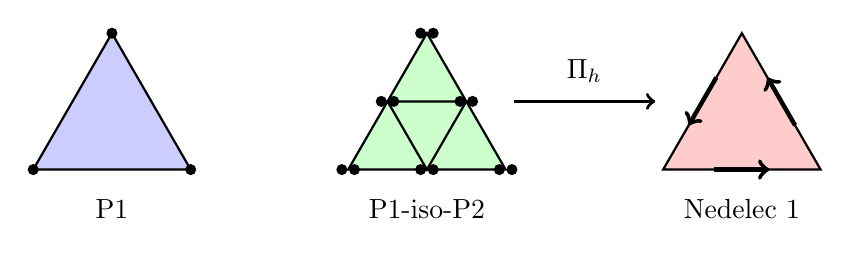
\begin{tikzpicture}

    % P1 element: vertex values
    \begin{scope}[shift={(0,0)}]
        \filldraw[fill=blue!20, cell] (0,0) -- (2,0) -- (1,1.732) -- cycle;
        \foreach \p in {(0,0), (2,0), (1,1.732)} {\scalardof{\p}}
        \node at (1,-0.5) {P1};
    \end{scope}

    % P1-iso-P2 element: vector values at the vertices and the edge midpoints
    \begin{scope}[shift={(4,0)}]
        \filldraw[fill=green!20, cell] (0,0) -- (2,0) -- (1,1.732) -- cycle;
        \draw[cell] (1,0) -- (1.5,0.866) -- (0.5,0.866) -- cycle;
        \foreach \p in {(0,0), (2,0), (1,1.732), (1,0), (0.5,0.866), (1.5,0.866)} {\vectordof{\p}}
        \node at (1,-0.5) {P1-iso-P2};
    \end{scope}

    % Reduction operator
    \draw[operator] (6.1,0.866) -- (7.9,0.866);
    \node at (7,1.25) {$\Pi_h$};

    % Nédélec element: tangential moments on the edges
    \begin{scope}[shift={(8,0)}]
        \filldraw[fill=red!20, cell] (0,0) -- (2,0) -- (1,1.732) -- cycle;
        \draw[edge dof] (0.65,0) -- (1.35,0);
        \draw[edge dof] (1.675,0.563) -- (1.325,1.169);
        \draw[edge dof] (0.675,1.169) -- (0.325,0.563);
        \node at (1,-0.5) {Nedelec 1};
    \end{scope}

\end{tikzpicture}
\end{document}
